\documentclass{article}
\usepackage{amsfonts}
\usepackage{graphicx}


\title{Pareto fronte v več dimenzijah}
\author{Klara Penko, Nejc Jenko}
\date{December 2021}


\begin{document}

\begin{titlepage}
    \maketitle
\end{titlepage}

\section{Definicija pareto fronte}
${\rm \textbf{Definicija 1}}$ Naj bo S prostor definiran z množico n dimenzij $\{d_{1},d_{2}\dots,d_{n}\}$ in D podmnožica množice S. Naj bo $p \in D$, podana z $p = (p_{1},p_{2},\dots,p_{n})$, kjer je $p_{i}$ vrednost v dimenziji $d_{i}$. Točka $p \in D$ \textbf{dominira} točko $q \in D$ na podprostoru $S'\subseteq S$, če v vsaki dimenziji $d_{i} \in S'$ velja $p_{i} \le q_{i}$ in v vsaj eni dimenziji $d_{j} \in S'$, $p_{j} < q_{j}$. 
\underline{\textbf{Pareto fronta}} prostora $S' \subseteq S$ je množica točk $D' \subseteq D,$ ki niso dominirane z nobeno točko v prostoru $S'$. \break
\break
${\rm \textbf{Primer v dveh dimenzijah}}$

 \begin{figure}[htbp]
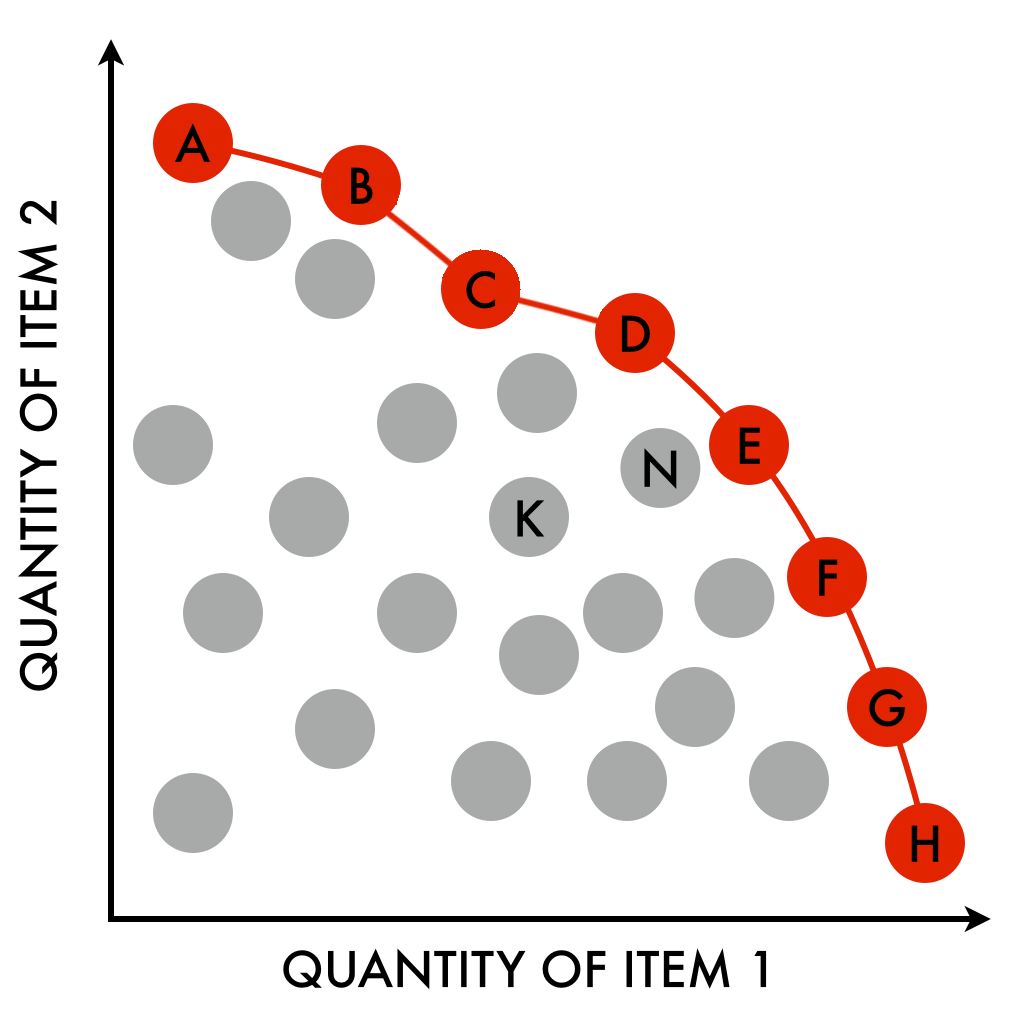
\includegraphics[width=4cm]{Slika_pareto_fronta.jpg}
\centering
\end{figure}

\section{Opis problema in načrt za nadaljnje delo}

Pri najinem projektu si bova ogledala Pareto fronte na d-dimenzionalnih (končnih?) množicah. Opazovala bova točke v d-dimenzionalnih kroglah in (hiper)kockah. Analizirala bova število točk na Pareto fronti in odvisnost od dimenzije d. Nato si bova pogledala še drugo in tretjo Pareto fronto ter n-to Pareto fronto, kjer iterativno n-krat iz množice odstraniš vse točke v Pareto fronti. Pri tem bova napisala program, ki nam iz poljubne dane množice točk vrne poljubno n-to Pareto fronto. S tem programom bova zaključke, do katerih sva prišla podkrepila ali pa ovrgla še eksperimentalno.




\end{document}
